\section*{Research Methodology}

The major research findings of this proposal are structured around three phases:  \textbf{(1) Data Preparation}, \textbf{(2) Model Development}, and \textbf{(3) Real-World Application Testing}.


\subsection*{Phase 1: Data Preparation and Feature Engineering}
This phase focuses on the meticulous preparation and structuring of the data required for model training. It involves collecting diverse and high-quality audio corpora for each language, encompassing a range of speakers, ages, and emotions. Essential annotations will specify speaker characteristics, emotions expressed, and the corresponding text. The corpora will be designed to represent various accents, dialects, and speaking styles within each language. Parallel corpora (audio and corresponding scripts) specific to different media (e.g., audiobooks, audio dramas, documentaries) will be collected to capture contextual variations. The data will be preprocessed to address inconsistencies and enhance overall quality through methods like noise reduction, normalization, and segmentation into individual utterances. Automated and manual feature extraction procedures will identify relevant acoustic cues (e.g., pitch, energy, spectral features) and linguistic features (e.g., phoneme duration, pause durations, tonal variations, prosodic contours), crucial for modeling language-specific prosody. The extracted features will be carefully represented in a manner suitable for the model architecture.

\subsection*{Phase 2: Model Development and Training}
In this phase, a novel multilingual TTS framework using a transformer-based architecture will be designed. This framework will incorporate a multimodal encoder to integrate linguistic information, speaker characteristics, and emotional cues. The architecture will include language-specific components to handle the unique prosodic and phonetic characteristics of each language (English, Bengali, and Chinese). The framework will be trained on the prepared corpora using appropriate optimization techniques and loss functions. Rigorous validation will be conducted using held-out portions of the data to evaluate the framework's generalization capabilities. Ongoing evaluation during the training process using relevant metrics (like MOS) will guide the development and refinement of the model. This phase emphasizes iterative model refinement and hyperparameter optimization guided by performance evaluations.

\subsection*{Phase 3: Real-World Application Testing and Evaluation}
This phase evaluates the practical usability of the developed framework. The trained model will be adapted to specific real-world applications (e.g., generating audio for audiobooks, audio dramas, and documentaries). User-friendly interfaces will be designed for potential deployment. A comprehensive evaluation, combining objective metrics (Mean Opinion Score, ASR error rate) and subjective assessments from expert panels (voice actors, linguists, and audio professionals), will be conducted to assess the framework's effectiveness and overall quality in each application context. This evaluation will focus on the naturalness, expressiveness, and cultural appropriateness of the synthesized voices, providing crucial feedback for iterative improvement.

\begin{center}
    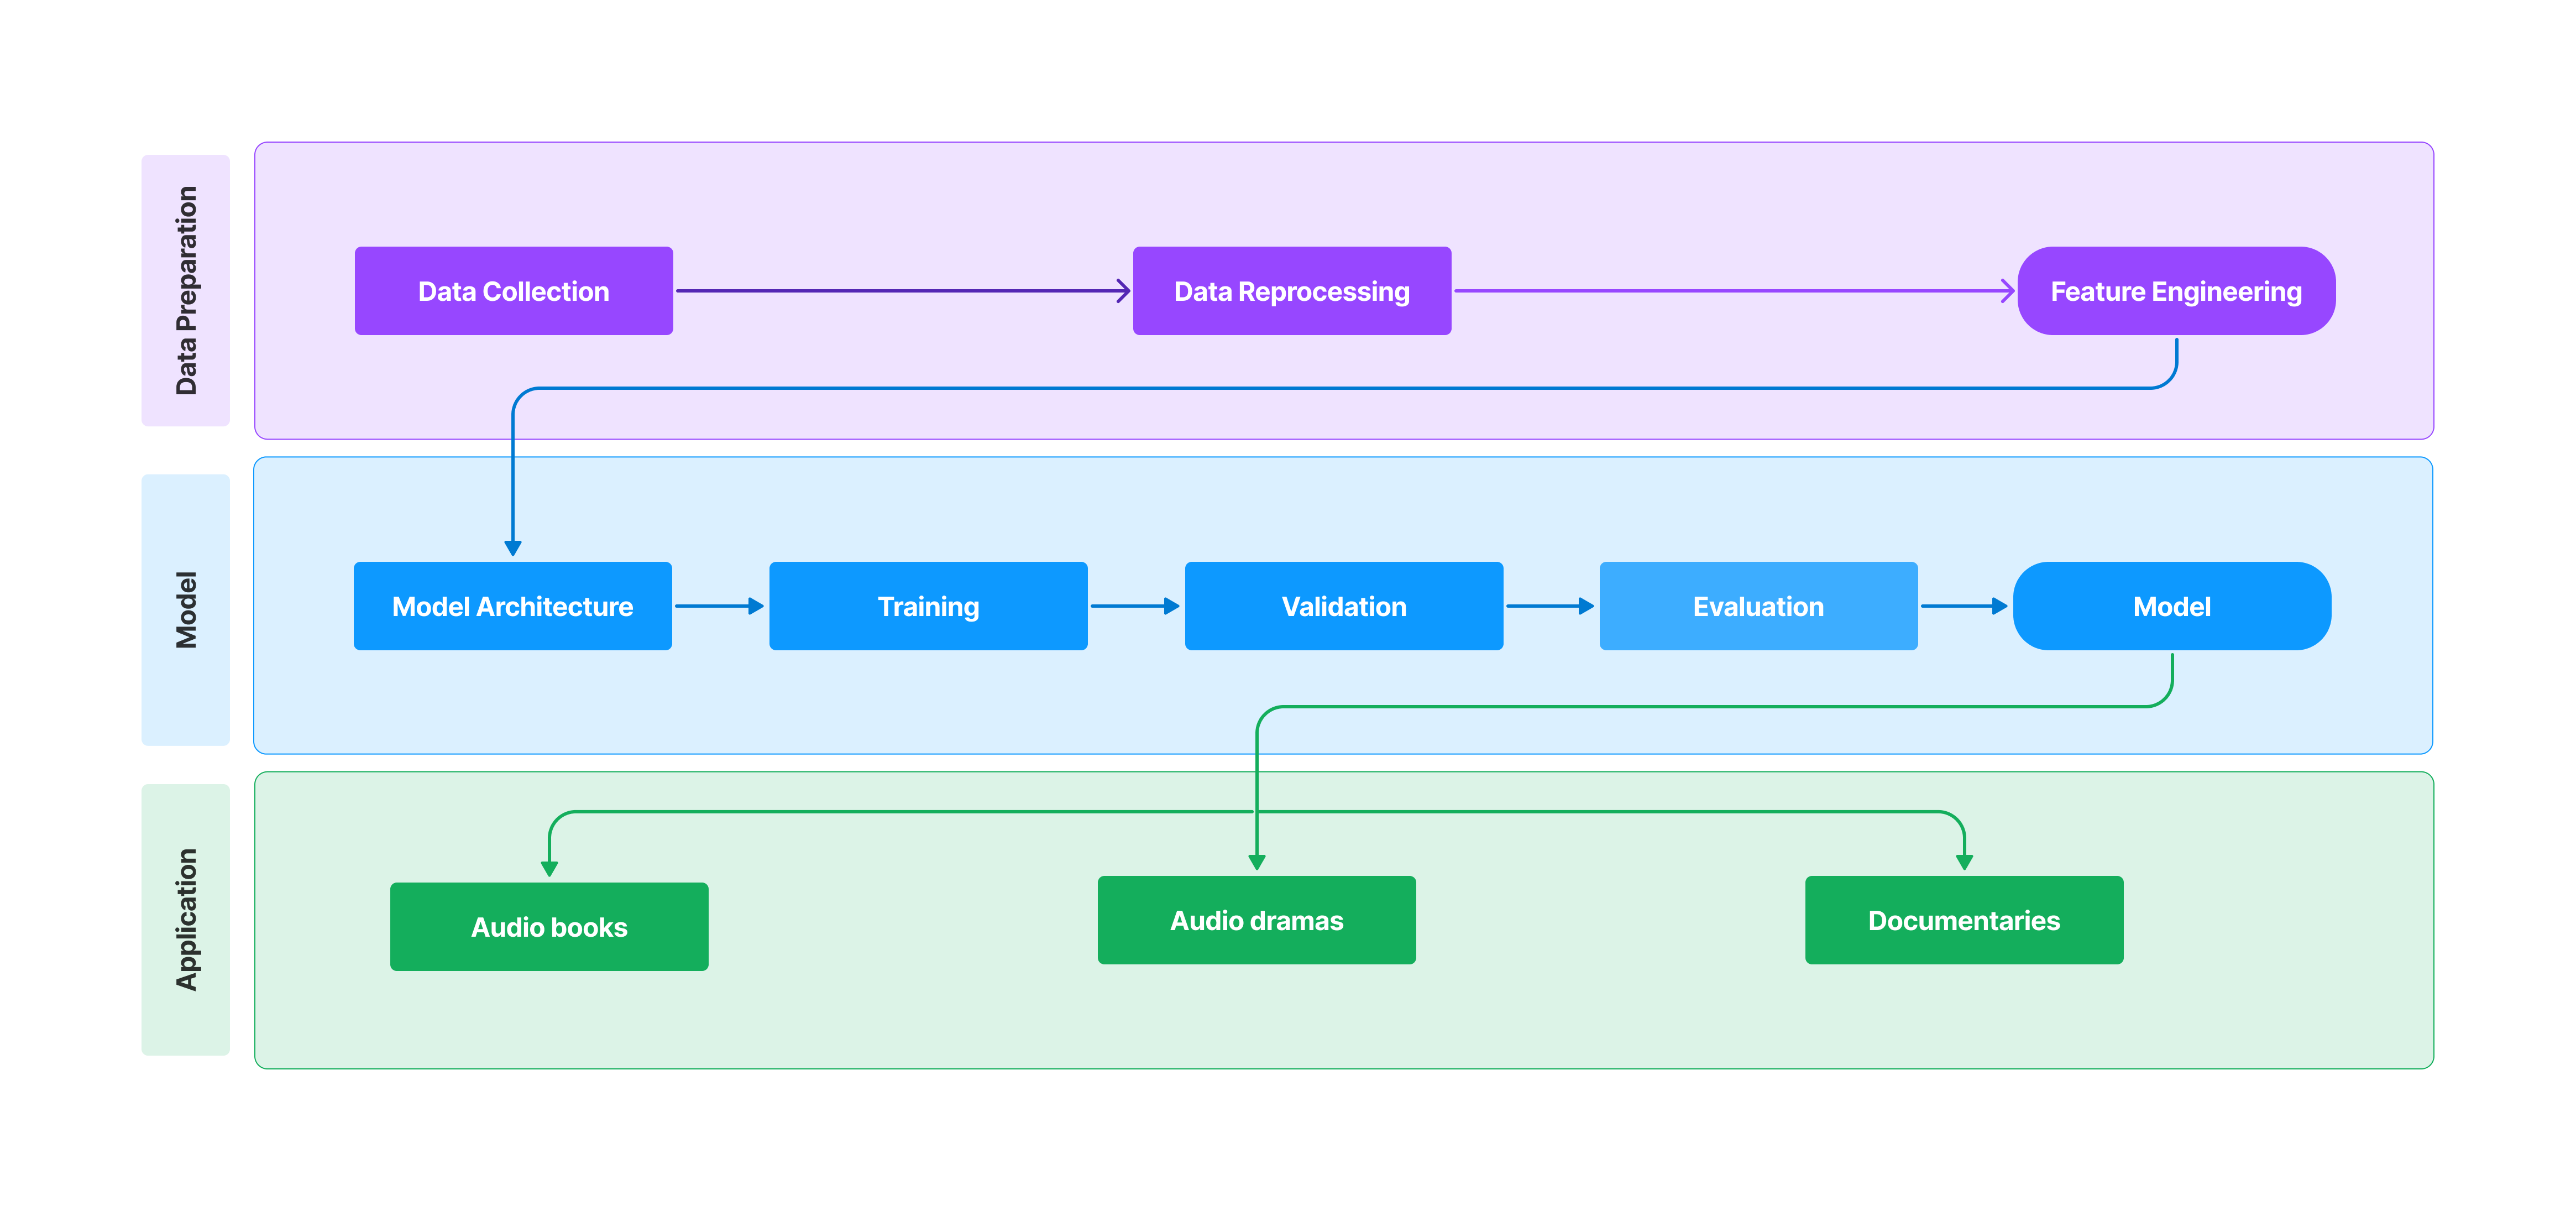
\includegraphics[width=1.0\textwidth]{research-flow.png}
    \captionof{figure}{Research flow}
\end{center}

This methodology employs a phased approach to develop a robust multilingual TTS framework. Data preparation, model development, and real-world testing phases ensure comprehensive evaluation and the framework's suitability for applications like audiobooks and documentaries. The approach prioritizes diverse data, language-specific modeling, and expert evaluation to create a high-quality, practical system.